\documentclass[14pt,pdf,hyperref={unicode}]{beamer}

% \documentclass[aspectratio=43]{beamer}
% \documentclass[aspectratio=1610]{beamer}
% \documentclass[aspectratio=169]{beamer}

\usepackage{lmodern}

% подключаем кириллицу 
\usepackage[T2A]{fontenc}
\usepackage[utf8]{inputenc}
\usepackage{listings}
\usepackage{graphicx}
\usepackage{hyperref}

% отключить клавиши навигации
\setbeamertemplate{navigation symbols}{}

% тема оформления
\usetheme{CambridgeUS}

% цветовая схема
\usecolortheme{seahorse}

\definecolor{light-gray}{gray}{0.90}

\lstset{basicstyle=\ttfamily,breaklines=true}

\title{Семинар №6}   
\subtitle{ФАКИ \the\year}
\author{Бирюков В. А.} 
\date{\today} 
% \logo{
\includegraphics[height=5mm]{images/logo.png}\vspace{-7pt}}

\begin{document}

\lstset{language=C}

% титульный слайд
\begin{frame}
\titlepage
\end{frame} 

\defverbatim[colored]\makeset{
\begin{lstlisting}[language=C++,basicstyle=\ttfamily,keywordstyle=\color{blue}]
void make_set(int X) {
  parent[X] = X;
}
\end{lstlisting}
}

\lstset{
  language=C,                % choose the language of the code
  keywordstyle=\color{blue},
  numbers=none,                   % where to put the line-numbers
  stepnumber=1,                   % the step between two line-numbers.        
  numbersep=5pt,                  % how far the line-numbers are from the code
  backgroundcolor=\color{light-gray},  % choose the background color. You must add \usepackage{color}
  showspaces=false,               % show spaces adding particular underscores
  showstringspaces=false,         % underline spaces within strings
  showtabs=false,                 % show tabs within strings adding particular underscores
  tabsize=2,                      % sets default tabsize to 2 spaces
  captionpos=b,                   % sets the caption-position to bottom
  breaklines=true,                % sets automatic line breaking
  breakatwhitespace=true,         % sets if automatic breaks should only happen at whitespace
}





\section{Переменные}
\begin{frame}
\begin{center}
\begin{beamercolorbox}[sep=8pt,center]{part
title}
\usebeamerfont{part title}\insertsection
\end{beamercolorbox}
\end{center}
\end{frame}



\begin{frame}
\frametitle{Переменные} 
\begin{center}
\begin{itemize}
\item В языке C все переменные нужно объявить перед использованием
\item При объявлении -- выделяется память под переменную
\item Области видимости переменной
\item Название переменной может содержать латинские буквы, цифры и \_
\item Название переменной не может начинаться с цифры
\end{itemize}
\end{center}
\end{frame}


\begin{frame}
\frametitle{Базовые типы}
\frametitle{Целочисленные типы} 
\begin{center}
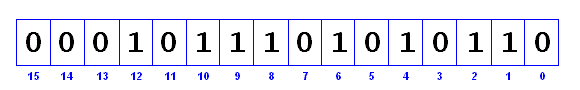
\includegraphics[scale=0.5]{bit_positions.png}
\end{center}
Число бит на тип зависит от компилятора. Обычные значения такие:
\begin{center}
\begin{tabular}{ l c l }
  Название типа & Число бит & Макс. значения \\
  char & 8 & 0..255 \\
  short & 16 & -32768..32767 \\
  int & 32 & $-2 \cdot 10^9$ ..$+2 \cdot 10^9$ \\
  long & 32& $-2 \cdot 10^9$ ..$+2 \cdot 10^9$ \\
  long long & 64 & $-2^{64}$ ..$+2^{64}-1$ \\
\end{tabular}
\end{center}
\end{frame}

\begin{frame}
\frametitle{Базовые типы}
\frametitle{Беззнаковые целочисленные типы} 
Число бит на тип зависит от компилятора. Обычные значения такие:
\begin{center}
\begin{tabular}{ l c l }
  Название типа & Число бит & Макс. значения \\
  unsigned short & 16 & 0..65535 \\
  unsigned int & 32 & $0$ ..$+4 \cdot 10^9$ \\
  unsigned long & 32& $0$ ..$+4 \cdot 10^9$ \\
  unsigned long long & 64 & $0$ ..$+2^{65}-1$ \\
\end{tabular}
\end{center}
sizeof() -- размер файла в байтах
\end{frame}


\begin{frame}
\frametitle{Базовые типы}
\frametitle{Типы чисел с плавающей точкой} 
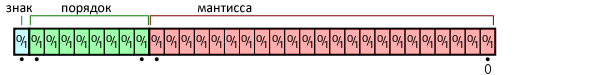
\includegraphics[scale=0.6]{floats.png}
\begin{center}
\begin{tabular}{ l c l }
  Название типа & Число бит & Макс. значения \\
  float & 32 & $10^{-38}$..$10^{+38}$ \\
  double & 64 & $10^{-308}$..$10^{+308}$ \\
\end{tabular}
\end{center}
Обычно используется double, так как float может недостаточно точен
\end{frame}



\begin{frame}
\frametitle{Вывод в stdout. Функция printf.}
printf(строка форматирования, пер1, пер2, ...)
\begin{center}
\begin{tabular}{ l l l }
  Обозначение & Типы & Пример \\
  d или i & Целочисленные типы & 392 \\
  f & Типы с плавающей точкой & 392.5 \\
  e & Научная нотация & 3.9265e+2 \\
  c & Символ & a \\
  s & Строка & HelloMipt! \\
\end{tabular}
\end{center}
\end{frame}



\begin{frame}
\frametitle{Базовые операторы}
\frametitle{Приоритет операторов}
\begin{center}
\begin{enumerate}
\item (), []
\item ++, --, +, -(унарные), sizeof
\item *, /, \%
\item +, -
\item >,<,<=,>=
\item ==, !=
\item \&, |, \&\&, ||
\item =, +=, и т.д.
\end{enumerate}
\end{center}
Приоритет операторов C подробнее:\\
\href{http://ru.cppreference.com/w/c/language/operator_precedence}
{\textcolor{red}{ru.cppreference.com/w/c/language/operator\_precedence}}
\end{frame}



\section{Управляющие конструкции}
\begin{frame}
\begin{center}
\begin{beamercolorbox}[sep=8pt,center]{part
title}
\usebeamerfont{part title}\insertsection
\end{beamercolorbox}
\end{center}
\end{frame}



\begin{frame}
\frametitle{Базовые управляющие конструкции} 
\framesubtitle{Цикл while}

\lstset{
  language=C,                % choose the language of the code
  keywordstyle=\color{blue},
  numbers=none,                   % where to put the line-numbers
  stepnumber=1,                   % the step between two line-numbers.        
  numbersep=5pt,                  % how far the line-numbers are from the code
  backgroundcolor=\color{light-gray},  % choose the background color. You must add \usepackage{color}
  showspaces=false,               % show spaces adding particular underscores
  showstringspaces=false,         % underline spaces within strings
  showtabs=false,                 % show tabs within strings adding particular underscores
  tabsize=2,                      % sets default tabsize to 2 spaces
  captionpos=b,                   % sets the caption-position to bottom
  breaklines=true,                % sets automatic line breaking
  breakatwhitespace=true,         % sets if automatic breaks should only happen at whitespace
}

\lstinputlisting{./programms/code_while.c}

Напечатает 1 2 3 

\end{frame}

\begin{frame}
\frametitle{Базовые управляющие конструкции} 
\framesubtitle{Цикл do while}

\lstset{
  language=C,                % choose the language of the code
  keywordstyle=\color{blue},
  numbers=none,                   % where to put the line-numbers
  stepnumber=1,                   % the step between two line-numbers.        
  numbersep=5pt,                  % how far the line-numbers are from the code
  backgroundcolor=\color{light-gray},  % choose the background color. You must add \usepackage{color}
  showspaces=false,               % show spaces adding particular underscores
  showstringspaces=false,         % underline spaces within strings
  showtabs=false,                 % show tabs within strings adding particular underscores
  tabsize=2,                      % sets default tabsize to 2 spaces
  captionpos=b,                   % sets the caption-position to bottom
  breaklines=true,                % sets automatic line breaking
  breakatwhitespace=true,         % sets if automatic breaks should only happen at whitespace
}

\lstinputlisting{./programms/code_do_while.c}

Напечатает 1 2 3 

\end{frame}

\begin{frame}
\frametitle{Базовые управляющие конструкции} 
\framesubtitle{Цикл for}

\lstset{
  language=C,                % choose the language of the code
  keywordstyle=\color{blue},
  numbers=none,                   % where to put the line-numbers
  stepnumber=1,                   % the step between two line-numbers.        
  numbersep=5pt,                  % how far the line-numbers are from the code
  backgroundcolor=\color{light-gray},  % choose the background color. You must add \usepackage{color}
  showspaces=false,               % show spaces adding particular underscores
  showstringspaces=false,         % underline spaces within strings
  showtabs=false,                 % show tabs within strings adding particular underscores
  tabsize=2,                      % sets default tabsize to 2 spaces
  captionpos=b,                   % sets the caption-position to bottom
  breaklines=true,                % sets automatic line breaking
  breakatwhitespace=true,         % sets if automatic breaks should only happen at whitespace
}

\lstinputlisting{./programms/code_for.c}

Напечатает 1 2 3 

\end{frame}




\begin{frame}
\frametitle{Управляющие конструкции} 
\framesubtitle{Оператор break}

\lstset{
  language=C,                % choose the language of the code
  keywordstyle=\color{blue},
  numbers=none,                   % where to put the line-numbers
  stepnumber=1,                   % the step between two line-numbers.        
  numbersep=5pt,                  % how far the line-numbers are from the code
  backgroundcolor=\color{light-gray},  % choose the background color. You must add \usepackage{color}
  showspaces=false,               % show spaces adding particular underscores
  showstringspaces=false,         % underline spaces within strings
  showtabs=false,                 % show tabs within strings adding particular underscores
  tabsize=2,                      % sets default tabsize to 2 spaces
  captionpos=b,                   % sets the caption-position to bottom
  breaklines=true,                % sets automatic line breaking
  breakatwhitespace=true,         % sets if automatic breaks should only happen at whitespace
}

\lstinputlisting{./programms/code_break.c}
\end{frame}

\begin{frame}
\frametitle{Управляющие конструкции} 
\framesubtitle{Оператор continue}

\lstset{
  language=C,                % choose the language of the code
  keywordstyle=\color{blue},
  numbers=none,                   % where to put the line-numbers
  stepnumber=1,                   % the step between two line-numbers.        
  numbersep=5pt,                  % how far the line-numbers are from the code
  backgroundcolor=\color{light-gray},  % choose the background color. You must add \usepackage{color}
  showspaces=false,               % show spaces adding particular underscores
  showstringspaces=false,         % underline spaces within strings
  showtabs=false,                 % show tabs within strings adding particular underscores
  tabsize=2,                      % sets default tabsize to 2 spaces
  captionpos=b,                   % sets the caption-position to bottom
  breaklines=true,                % sets automatic line breaking
  breakatwhitespace=true,         % sets if automatic breaks should only happen at whitespace
}

\lstinputlisting{./programms/code_continue.c}
\end{frame}





\section{Массивы и строки}
\begin{frame}
\begin{center}
\begin{beamercolorbox}[sep=8pt,center]{part
title}
\usebeamerfont{part title}\insertsection
\end{beamercolorbox}
\end{center}
\end{frame}


\begin{frame}[fragile]
\frametitle{Массивы} 
\framesubtitle{Примеры}
Объявление:\\
\begin{lstlisting}
int array[10];
float average_temperature[12];
\end{lstlisting}
Доступ к элементу:\\
Нумерация в массиве начинается с 0\\
\begin{lstlisting}
printf("%d\n", array[9]);
average_temperature[2] = 5.2;
\end{lstlisting}
\end{frame}

\begin{frame}[fragile]
\frametitle{Массивы} 
\framesubtitle{Инициализация}
\begin{lstlisting}
int array[10];
for (int i = 0; i < 10; ++i) {
    array[i] = /* something */;
}
\end{lstlisting}
Или так:\\
\begin{lstlisting}
int array[5] = {1, 1, 2, 3, 5};
\end{lstlisting}
\end{frame}

\begin{frame}[fragile]
\frametitle{Массивы} 
\framesubtitle{Массивы в памяти}
\begin{center}
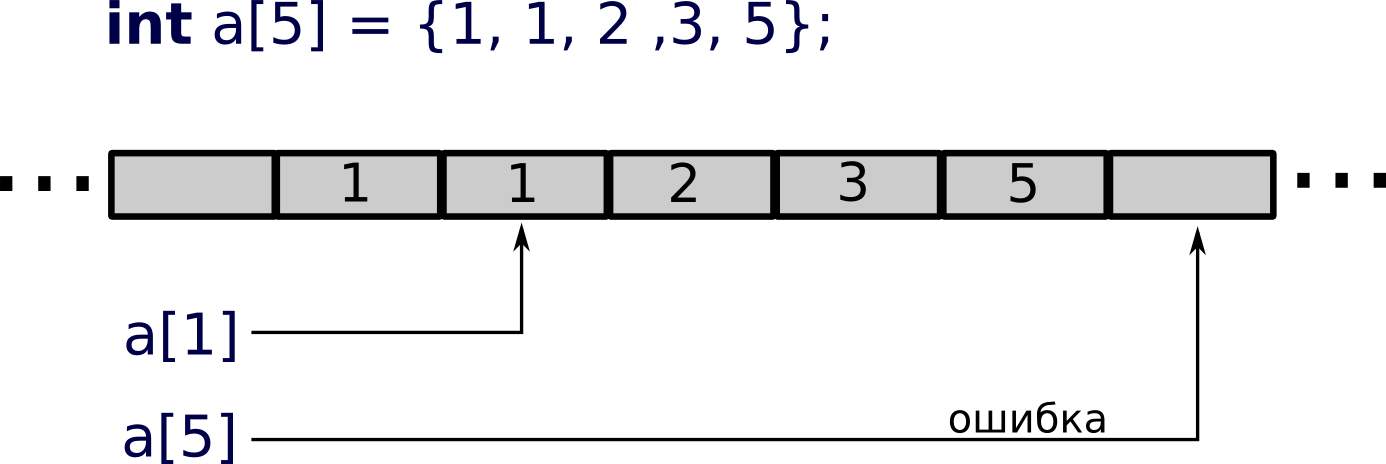
\includegraphics[width=0.95\linewidth]{images/array_in_memory.png}
\end{center}
\end{frame}




\begin{frame}[fragile]
\begin{center}
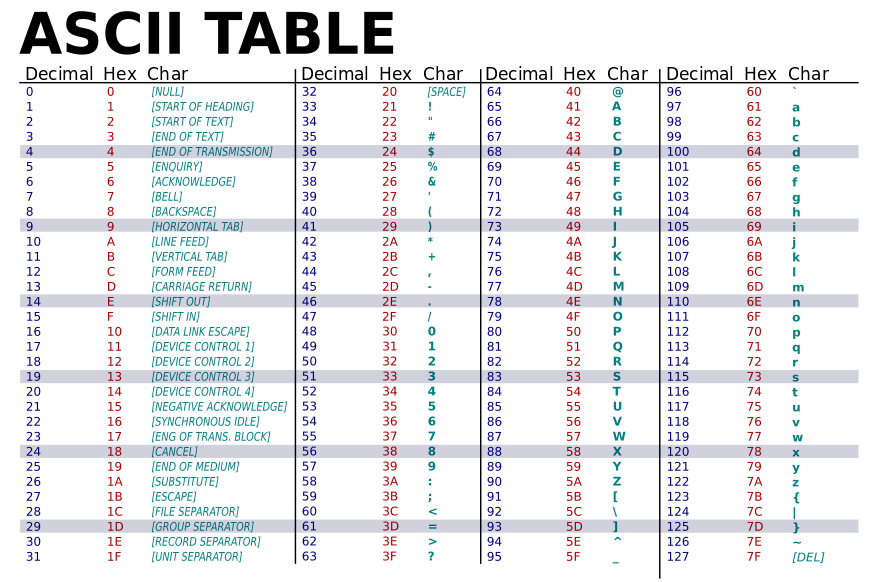
\includegraphics[width=1.02\linewidth]{images/ascii.png}
\end{center}
\end{frame}



\begin{frame}[fragile]
\frametitle{Строки} 
\framesubtitle{Инициализация}
\begin{lstlisting}
int string[10];
for (int i = 0; i < 10; ++i) {
    string[i] = /* something */;
}
\end{lstlisting}
Или так:\\
\begin{lstlisting}
int string[10] = {'h', 'e', 'l', 'l', 'o', '\0', 'a', 'b', 'c', 'd'};
\end{lstlisting}
Или так:\\
\begin{lstlisting}
int string[10] = "hello";
\end{lstlisting}
\end{frame}

\begin{frame}[fragile]
\frametitle{Строки} 
\framesubtitle{Строки в памяти}
\begin{center}
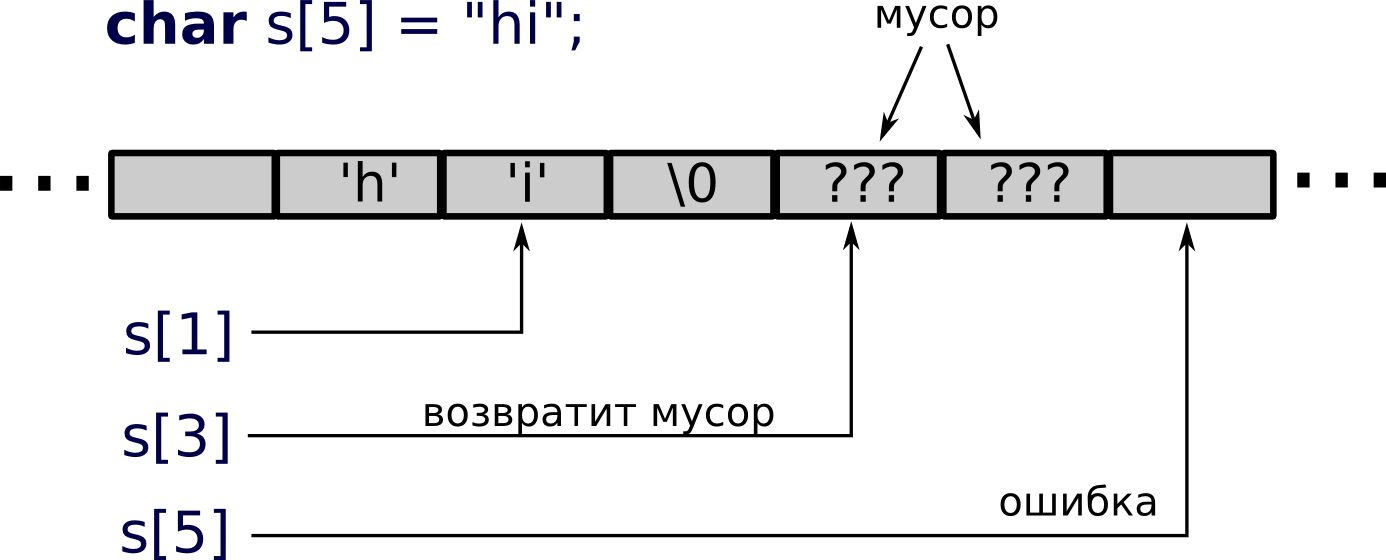
\includegraphics[width=0.95\linewidth]{images/string_in_memory.png}
\end{center}
\end{frame}



\begin{frame}[fragile]
\frametitle{Функции для работы со строками} 
Чтение строки:
\begin{lstlisting}
char string[10];
scanf("%10s", string);
\end{lstlisting}
Длина строки:
\begin{lstlisting}
#include <string.h>
char string[10] = "hello";
int n = strlen(string);
\end{lstlisting}
\end{frame}

\begin{frame}[fragile]
\frametitle{Функции для работы со строками} 
\begin{lstlisting}
#include <string.h>
char s1[10] = "hi";
char s2[10] = "world";
\end{lstlisting}
Копирование строки s2 в строку s1:
\begin{lstlisting}
strcpy(s1, s2);
\end{lstlisting}
Конкатенация строки s2 в строку s1:
\begin{lstlisting}
strcat(s1, s2);
\end{lstlisting}
\end{frame}









\section{Функций}
\begin{frame}
\begin{center}
\begin{beamercolorbox}[sep=8pt,center]{part
title}
\usebeamerfont{part title}\insertsection
\end{beamercolorbox}
\end{center}
\end{frame}


\begin{frame}[fragile]
\frametitle{Объявление функций(прототипы функций)} 
\begin{itemize}
\item Как и переменная, функция также должна объявлена перед использованием
\item Определение функции называется прототипом функции
\item Пример прототипа:\\
\begin{lstlisting}
int sum (int a, int b)
\end{lstlisting}
или:
\begin{lstlisting}
int sum (int , int)
\end{lstlisting}
\end{itemize}
\end{frame}


\begin{frame}[fragile]
\frametitle{Вызов функций} 
\begin{itemize}
\item Примеры вызова функции:\\
Функция, определяемая пользователем:\\
\begin{lstlisting}
sum(a, b)
\end{lstlisting}
Библиотечные функции:\\
\begin{lstlisting}
sqrt(x)
\end{lstlisting}
\begin{lstlisting}
printf("%d\n", a)
\end{lstlisting}
\end{itemize}
\end{frame}



\begin{frame}[fragile]
\frametitle{Определение функции} 
\begin{center}
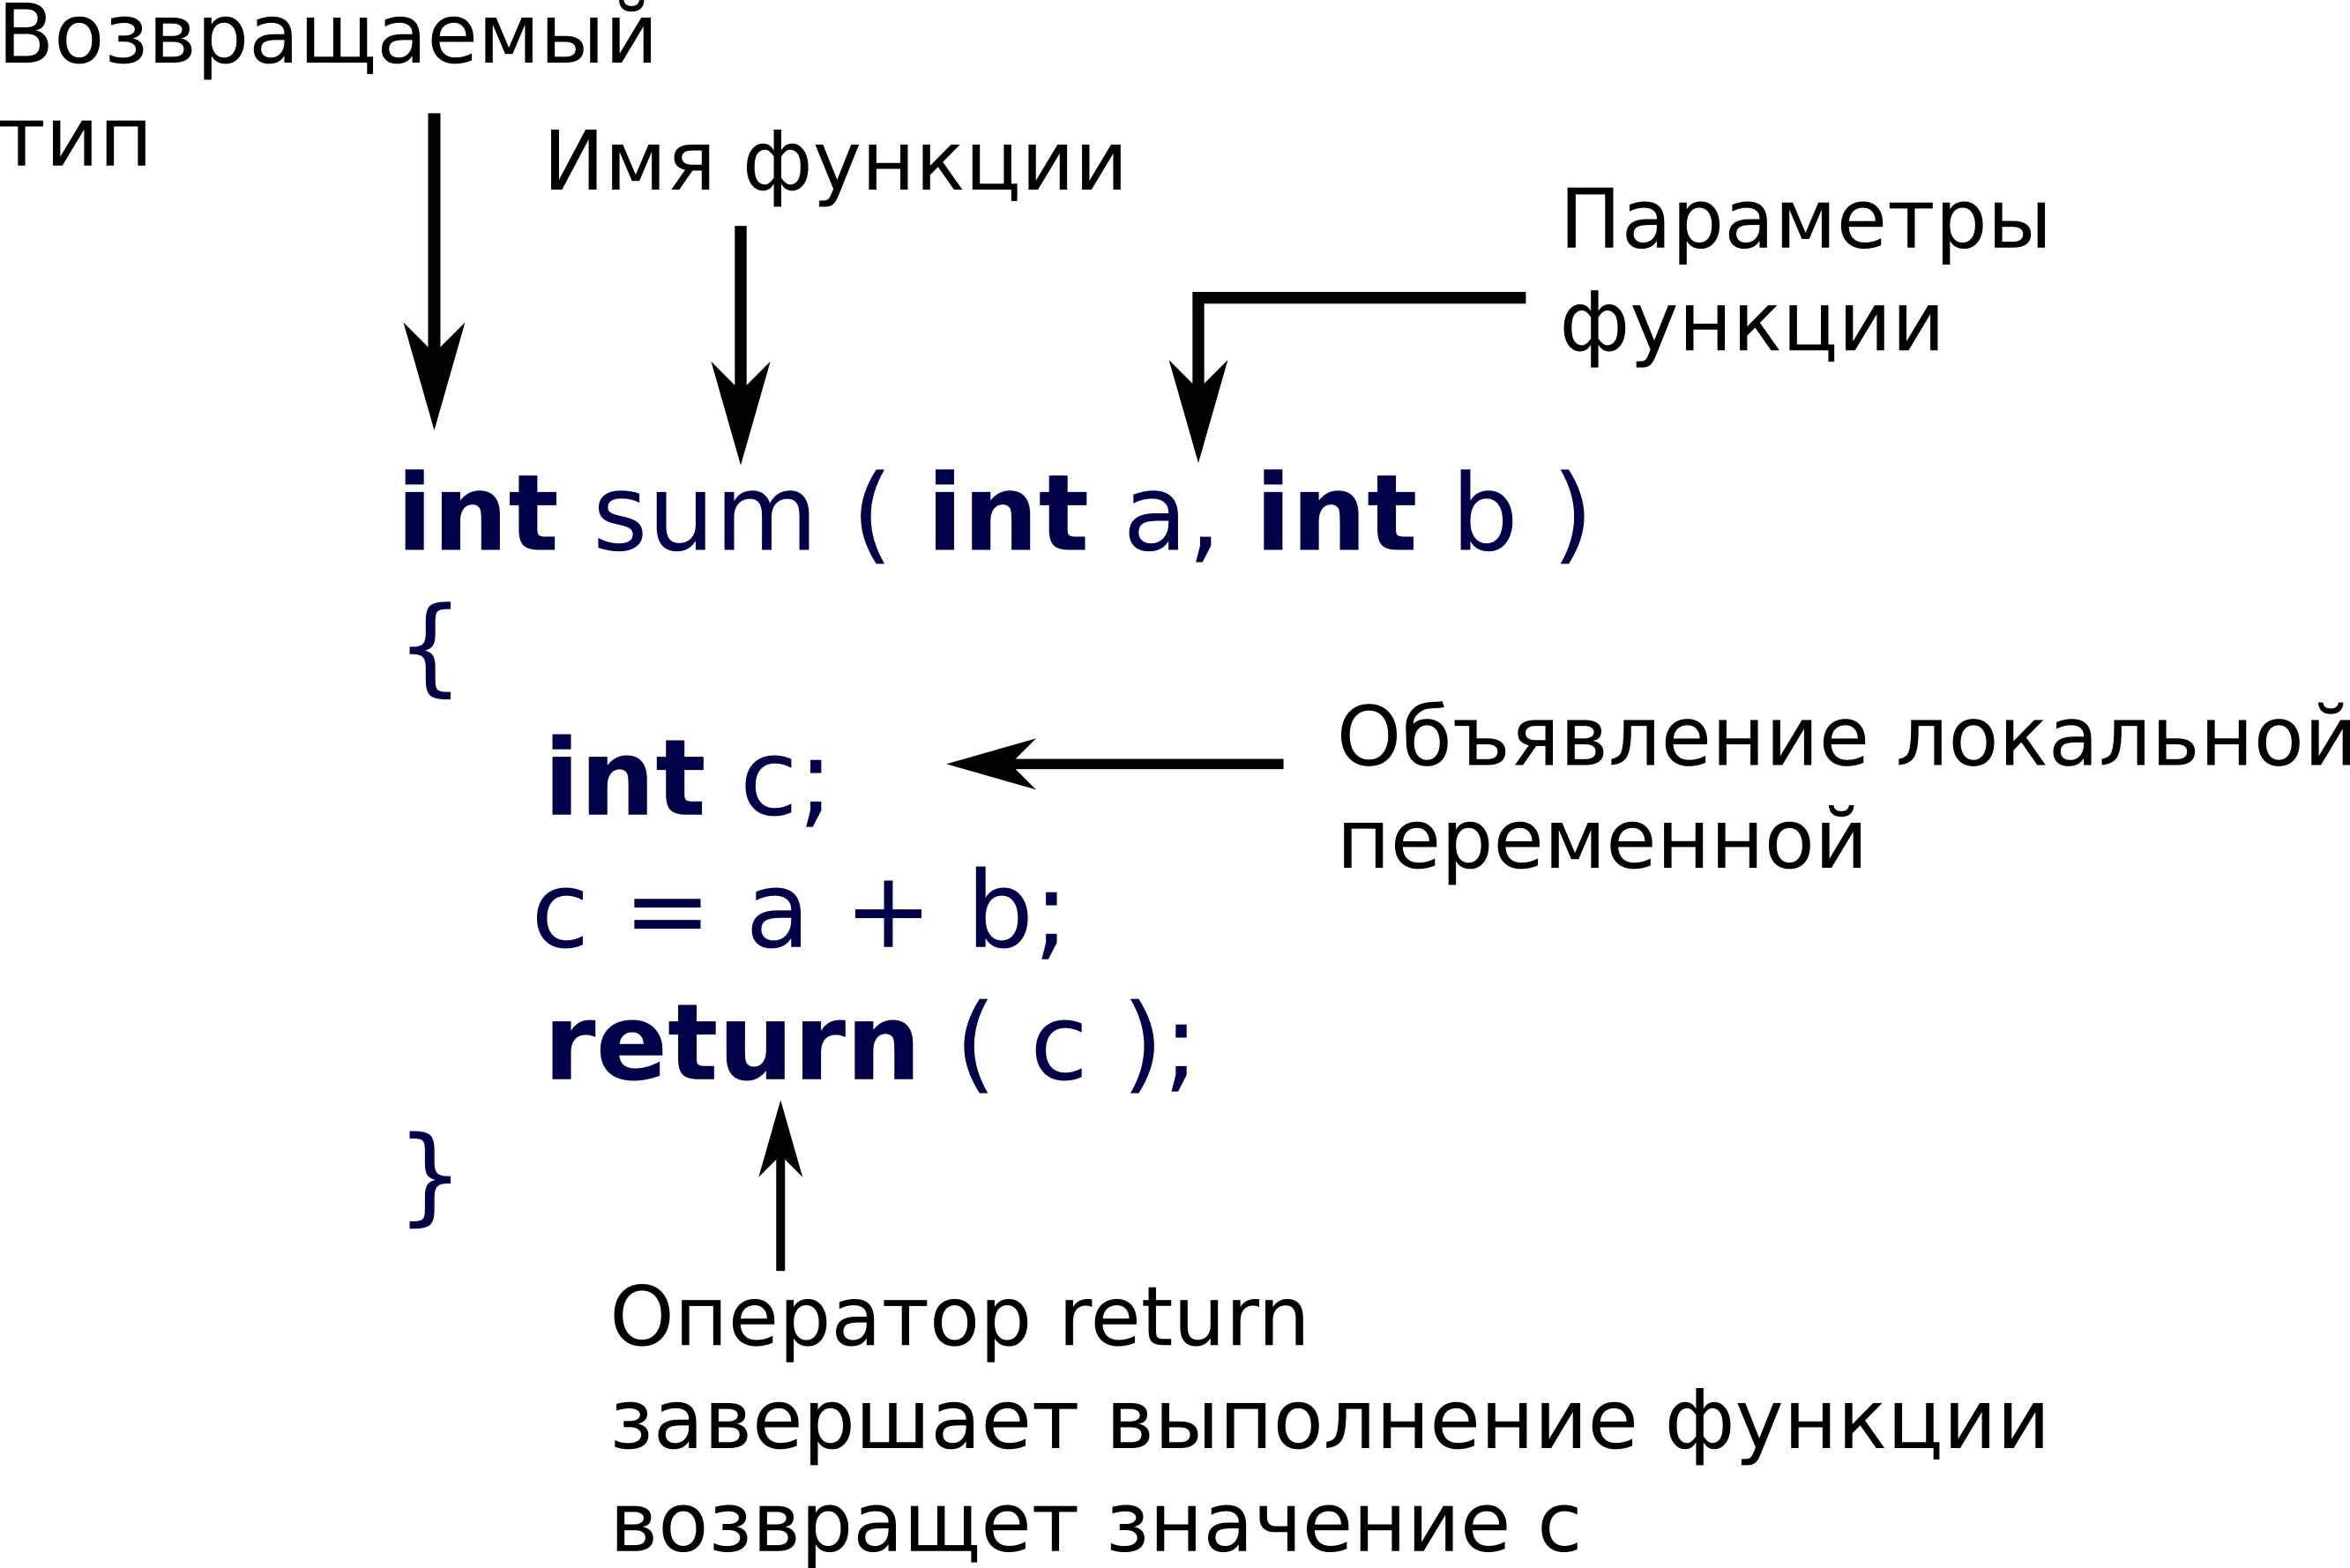
\includegraphics[width=0.8\linewidth]{images/function_syntax.png}
\end{center}
\end{frame}

\begin{frame}[fragile]
\frametitle{Функции} 
\begin{center}
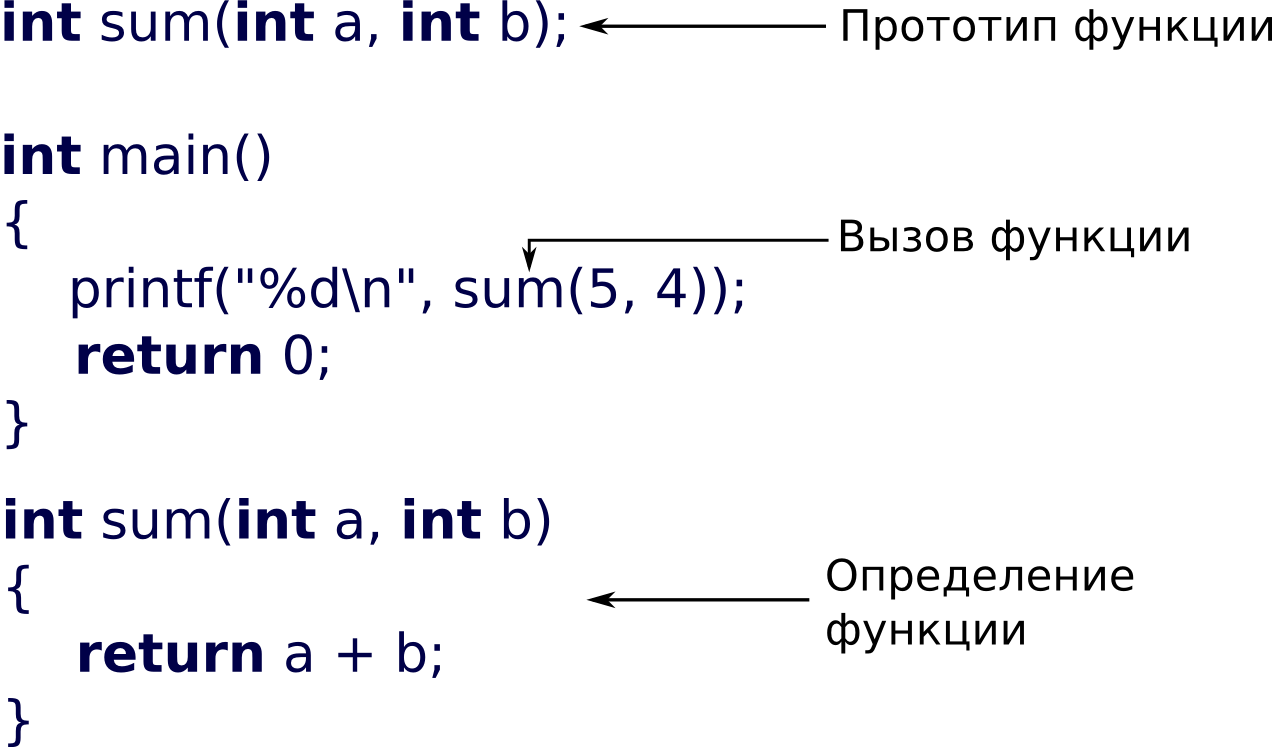
\includegraphics[width=0.8\linewidth]{images/function_summary.png}
\end{center}
\end{frame}

\begin{frame}[fragile]
\frametitle{Функции} 
\begin{center}
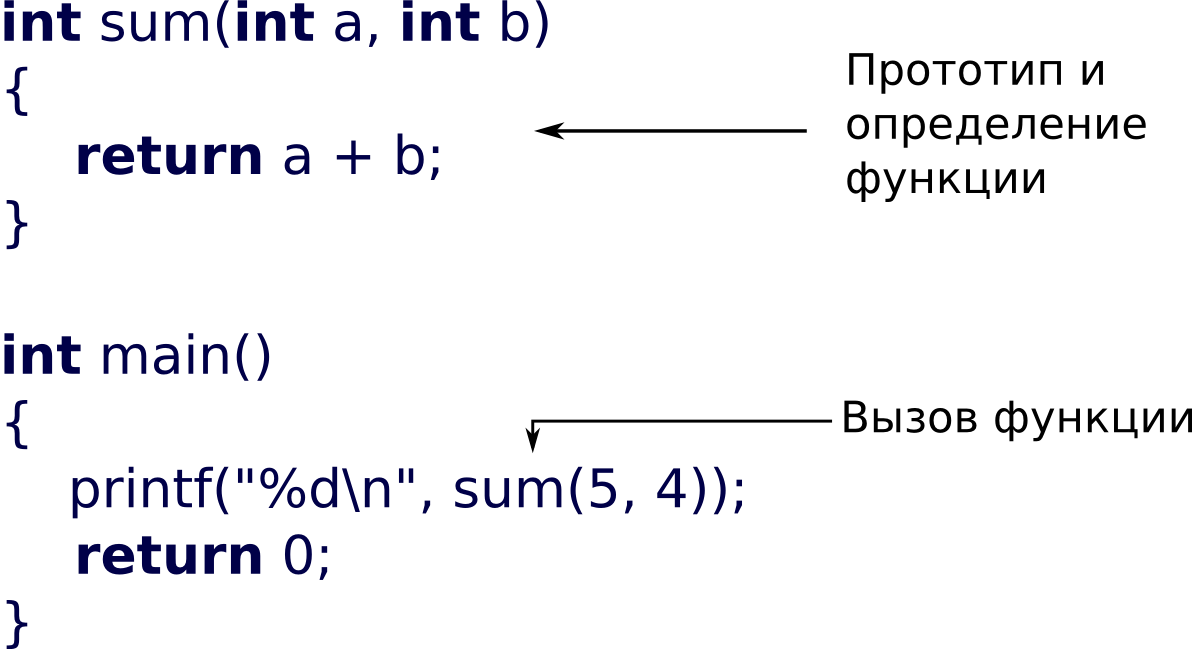
\includegraphics[width=0.8\linewidth]{images/function_summary2.png}

\end{center}
\end{frame}




\section{Области видимости переменных}
\begin{frame}
\begin{center}
\begin{beamercolorbox}[sep=8pt,center]{part
title}
\usebeamerfont{part title}\insertsection
\end{beamercolorbox}
\end{center}
\end{frame}

\begin{frame}[fragile]
\frametitle{Области видимости переменных} 
\begin{itemize}
\item Область видимости -- область программы, в пределах которой имя некоторой переменной продолжает быть связанным с этой переменной и возвращать её значение.
\item Глобальная переменная -- объявляются вне всех функций и доступны отовсюду
\item Локальная переменная --  объявляются внутри блока и недоступны вне его
\end{itemize}
\end{frame}

\begin{frame}[fragile]
\frametitle{Области видимости переменных} 
Функция определяет собственную (локальную) область видимости, куда входят:
\begin{enumerate}
\item Глобальные переменные
\item Входные параметры
\item Переменные, которые объявляются в теле самой функции
\end{enumerate}
\end{frame}





\begin{frame}[fragile]
\frametitle{Материалы для подготовки} 
\begin{itemize}
\item Керниган, Ричи. Язык C
\item CS50 (перевод лекций есть в vk)
\item http://style.vdi.mipt.ru/  -- тренировка перед контрольной работой
\end{itemize}
\end{frame}



\end{document}
